% !TEX root = ../main.tex
\section{Findings for the Entire Population}
  
  This section will go through the results from the survey based on the entire population. 

  \todo[inline, color=blue!60]{The data used in this section are preprocessed. The procedures can be found in section.}
  \todo[inline, color=blue!60]{Skal treningsdata fjernes?}

	\subsection{Pattern Creation Time}
    When creating a pattern in the survey, both time used to create a pattern and the pattern created was recorded. The time used to create the pattern was recorded from the start when the grid appeared until the user submitted the pattern.

    Figure \ref{fig:avgpatterncreationtimepopulation} shows pattern creation time in seconds for the three pattern types, including the patterns created in the training mode. Looking at the average creation time, bank have the highest creation time of 10.43 seconds while patterns created for smartphones had an average creation time of 8.24 seconds. 

    Figure \ref{fig:patterncreationtimeexperience} shows the average pattern creation time in seconds for the entire population regards to participants experience with the Android Unlock Pattern. The graph shows that both patterns created for shopping account and banking account are not affected by the participants experience with the Android Unlock pattern. Both pattern types do not have any significant difference in average creation time regarding the participants experience. Looking at patterns created for smartphone and training, both have a significant difference in the average creation time regarding the participants experience with ALP. Smartphone have an average creation time of 7.62 seconds for participants experienced with ALP and an average creation time of 9.82 seconds for people not experienced with ALP. The significant difference in average creation time results in a difference of 2.2 seconds. The training patterns have a total difference in average creation time of 2.76 seconds.  

		\begin{figure}[H]
      \subfigure[Average pattern creation time (seconds)]{
        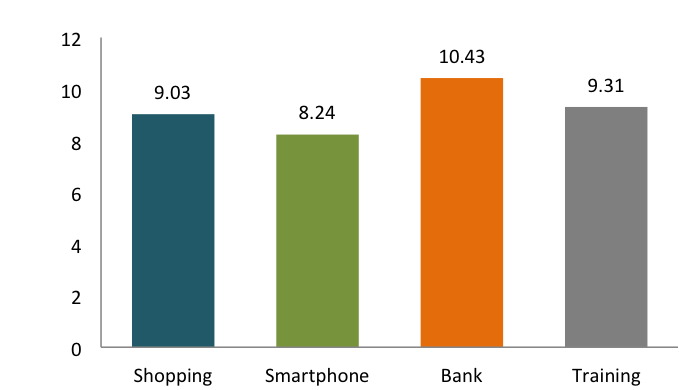
\includegraphics[scale=0.48]{pics/analysis/avgCreationTime.png}
        \label{fig:avgpatterncreationtimepopulation}
      }
      \subfigure[Creation time and experience with ALP]{
        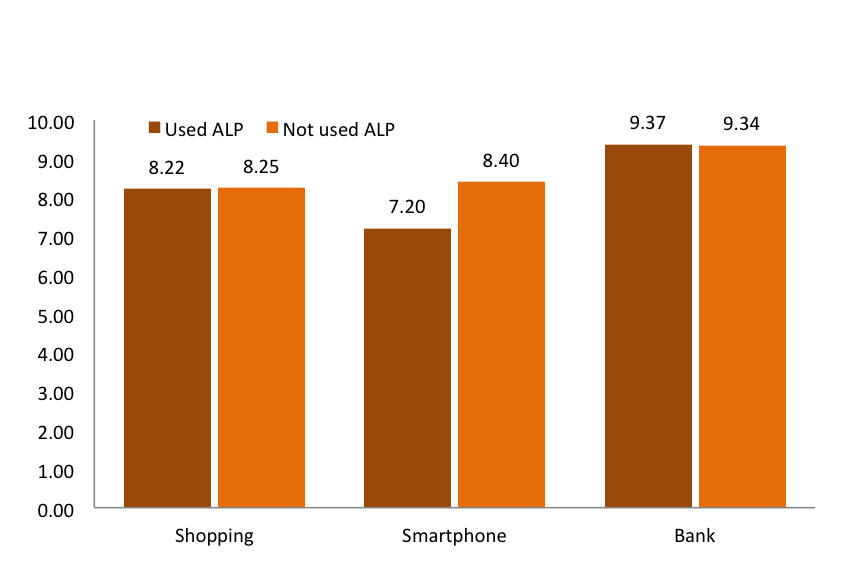
\includegraphics[width=0.48\textwidth]{pics/analysis/usedALPpatterncreationtime3.png}
        \label{fig:patterncreationtimeexperience}
      }
      \caption{Pattern creation time for the entire population}
      \label{fig:patterncreationtimepopulation}
    \end{figure}

	\subsection{Pattern Length}

    The pattern length are defined as the number of dots used to form a pattern. Each dot have a own sequence number and can only appear once. The minimum length of a pattern is 4 and the maximum length is 9. The number of unique patterns of all possible pattern lengths are described in table \ref{tab:combinations}. The pattern length are visualized in two different ways; the average pattern length and the distribution of pattern length.

    Figure \ref{fig:avgpatternlengthpopulation} shows the average pattern length in number of nodes for the three pattern types, including the patterns from the training mode. In the graph, the shape of the graph is skewed. There are indication that patterns created for bank have a higher average pattern length. The numbers from the graph also indicates that patterns created from smartphone has the smallest average pattern length. The difference in average pattern length for patterns created for smartphone and banking are 0.52 nodes. Patterns created for shopping account are slightly longer than patterns created for smartphones, but there are no significant difference between them. When looking away from the three main patterns, the training patterns have the shortest average pattern length of with a average length of 5.35 nodes. 

    \begin{figure}[H]
      \centering
      \subfigure[Average Pattern Length (nodes)]{
        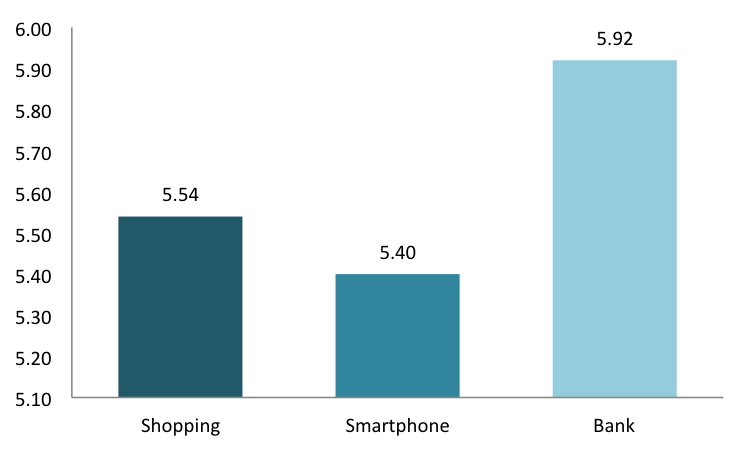
\includegraphics[scale=0.48]{pics/analysis/avgPatternLength.png}
        \label{fig:avgpatternlengthpopulation}
      }
      \subfigure[Pattern length distribution]{
        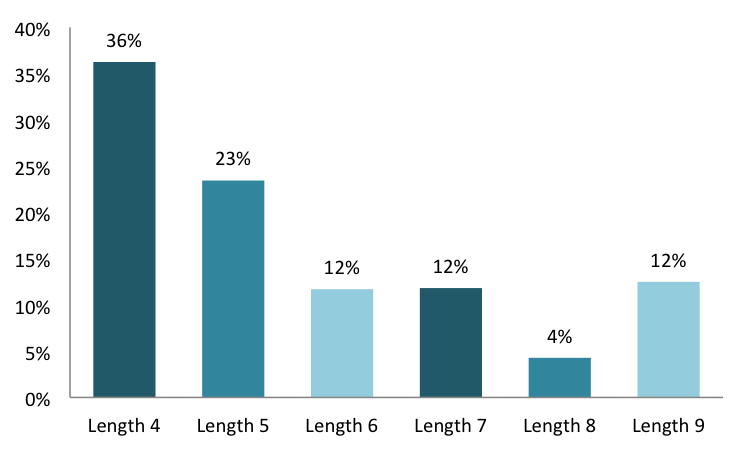
\includegraphics[width=0.48\textwidth]{pics/analysis/patternLength.png}
        \label{fig:patterndistpopulation}
      }
      \subfigure[Pattern length and type distribution]{
        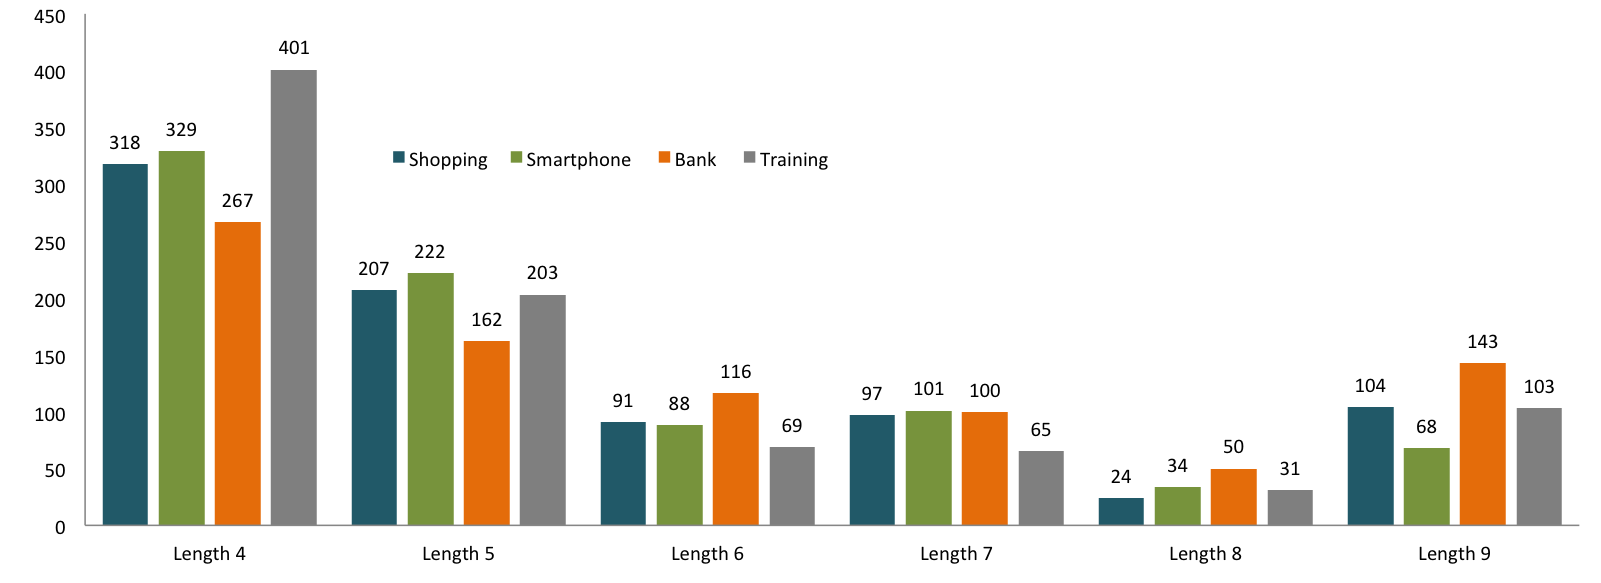
\includegraphics[width=\textwidth]{pics/analysis/patterntypePatternLength.png}
      \label{fig:patternTypePatternLength}
      }
      \caption{Pattern Length for the entire population}
      \label{fig:patternlengthpopulation}
    \end{figure}

    \clearpage

    The graph in Figure \ref{fig:patterndistpopulation} is a pattern length distribution indicating what pattern length that often are selected in the population. Figure \ref{fig:patternTypePatternLength} is a more detailed version of Figure \ref{fig:patterndistpopulation} showing the pattern distribution for all pattern types. Both graphs shows an indication that when the length increases the patterns of that length will occur less often. Both graphs also have a low frequency of pattern with length 8, where patterns of length 7 and 9 both have a higher frequency than patterns of length 8.

    By looking at the pattern length of each specific pattern type in Figure \ref{fig:patternTypePatternLength}, the distribution reflects the average pattern length. Patterns created for shopping account, smartphone and training have the majority of the patterns distributed over the shortest pattern length. Bank that had the highest average pattern length still have the majority of its patterns distributed over the lower pattern lengths, but do have the highest frequency of patterns of length 9. 

	\subsection{Pattern Complexity}

    Pattern complexity, e.g. pattern strength, is calculated from a mathematical formula that take into account the different aspects of visual complexity of patterns. The formula and parameters used are described in detail in Section \ref{sec:alp}. In short, the formula uses the size (number of nodes), physical size (length) of the pattern, number of intersections and number of overlaps. The minimum strength is 6.340 and the maximum strength is 46.807.

    Table \ref{tab:patternstrength} is a summary of all the parameters used in calculating the calculating the strength of the patterns in the entire population for all the different pattern types, including calculations of all the patterns collected. Since the pattern length are described in the previous subsection, this section will not comment on this again although the length of the pattern (e.g. size) are a part of calculating the strength. 

    \begin{table}[H]
    \centering
      \begin{tabular}{l || l | l | l || l}
        \hline
        {\bf Parameters} & {\bf Shopping} & {\bf Smartphone} & {\bf Bank} & {\bf All} \\ \hline
        \#Patterns & 841 & 842 & 838                  & 2521 \\
        Avg. Size & 5.541 & 5.398 & 5.920             & 5.619 \\ 
        Avg. Length & 5.050 & 4.920 & 5.666           & 5.212 \\
        \#Intersections & 177 & 149 & 363             & 689 \\
        Avg. Intersections & 0.210 & 0.1769 & 0.433   & 0.273 \\
        \#Overlaps & 15 & 12 & 19                     & 46 \\
        Avg. Overlaps & 0.0178 & 0.014 & 0.023        & 0.018 \\ \hline
        Avg. Strength & 13.440 & 12.837 & 15.514      & 13.928 \\ 
        Min strength & 6.340 & 6.340 & 6.340          & 6.340 \\
        Max strength & 44.441 & 43.187 & 44.441       & 44.441 \\ \hline
      \end{tabular}
      \caption{Pattern strength for all patterns types in the entire population}
      \label{tab:patternstrength}
    \end{table}

    The physical length, e.g. length, are increased when patterns creates lines between the nodes that are nor horizontal or vertical. A higher length are often correlated with the number of intersections and overlaps. Bank that have the highest strength do also have the highest average occurrences of intersections and overlaps, 0.433 and 0.023 respectively. 
    As seen before, patterns cerated for banking account have had a high pattern creation time and a high average pattern length that also are reflected in the average strength patterns created for banking account. The average strength for patterns created for banking account are 15.514.

    Smartphone is the pattern type with the lowest average strength excluding the patterns created for training purpose. The characteristics of patterns created for smartphones is that they have a short pattern length, the physical length are short, and the average occurrences of intersections and overlaps are low. The average number of occurrences of intersections and overlaps are 0.1769 and 0.014 respectively. The patterns created for smartphones gets an average strength score of 12.339. 

    Patterns created for shopping account are similar to patterns created for smartphone. All the parameters for the shopping account are slightly higher. The average strength for the patterns created for shopping account are 13.440.

    When looking at the maximum pattern strength of the all pattern strength, none of the respondents have managed to create a pattern with the highest possible pattern strength. The highest pattern strength in the data set is 44.441 where the maximum strength for patterns are 46.807. The patterns created for smartphones do not include patterns with strengths higher than 43.187 that is lower than the highest score in the dataset. 

    \todo[inline, color=red!70]{Må endre på avg. length for training i Tabell \ref{tab:patternstrength}}

	\subsection{Pattern Characteristics}

		\todo[inline, color=blue!60]{Sette inn association elements? Dette er en karakteristikk som befinner seg på tvers av populasjonen}

		\todo[inline, color=blue!60]{Sette inn noe om startpunkt?}

		\todo[inline, color=blue!60]{Passer 3-gram inn her?}

		%Figure: Number of unique patterns
    \begin{figure}[H]
      \centering
      \begin{minipage}[b]{0.40\linewidth}
      \centering
        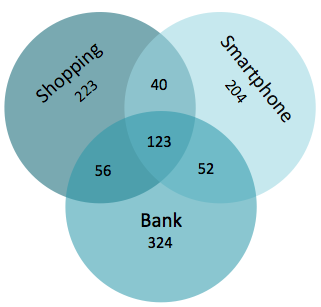
\includegraphics[scale=0.4]{pics/analysis/uniquePatternsVenn.png}
      \end{minipage}%
      \begin{minipage}[b]{0.30\linewidth}
        \centering
        \begin{tabular}{ c | c }
          \hline
          Shopping &  442 \\
          Smartphone & 419 \\
          Bank & 555 \\
          Training & 414 \\ \hline \hline
          All types & 1196 \\ \hline
        \end{tabular}
        \vspace{1cm}
      \end{minipage}
      \caption{Number of unique patterns}
      \label{fig:test}
    \end{figure}
    

  \subsection{Association Elements} \label{sec:associationelements}
    An association element are something someone or something you know and can use as a element so the process of remembering can be easier. This is a known technique used in alphanumeric passwords and PIN codes. Alphanumeric passwords are often known to contain personal information like names, dates, and objects close to the user. The same with PIN codes where the the technique of using codes forming a date often occurs. 
    \todo{Kilder} 

    Going through the alphabet, I was able to find 11 patterns having the same visual representation as letters from the alphabet. Out of the 12 letters, 9 patterns had a significant number of appearances in the data set. By iterating through a list of sequences forming a letter, I was able to find 385 out of 3393 patterns in the dataset matching one of the 13 letters in the alphabet. The number of patterns occurred to match a letter from the alphabet constitutes 11.4\% of all patterns in the data set. 

    Figure \ref{fig:associationpatterns} shows the 8 most common patterns having the same visual representation as letters from the alphabet. Beside the letters C, L, M,N, O, S, U and Z, letters like G, J and W also appeared in the data set.

    \clearpage

      \begin{figure}[H]
        \centering
        \vspace{1.5cm}

        \subfigure[The letter C]{
          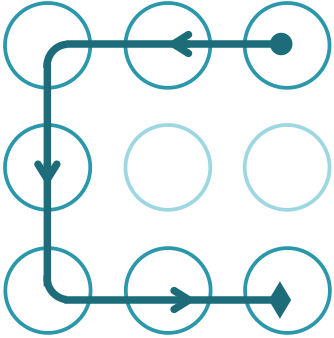
\includegraphics[width=0.27\textwidth]{pics/letters/bokstavenC.png}\hspace{0.6cm}
        }
        \subfigure[The letter L (big)]{
          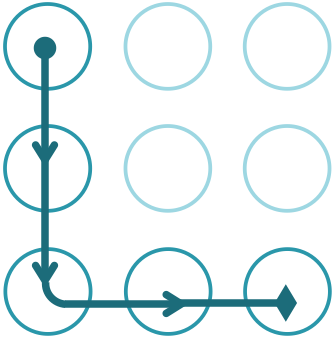
\includegraphics[width=0.27\textwidth]{pics/letters/bokstavenL.png}\hspace{0.6cm}
        }
        \subfigure[The letter L (small)]{
          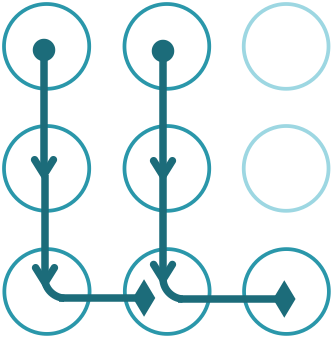
\includegraphics[width=0.27\textwidth]{pics/letters/bokstavenLitenL.png}
        }

        \vspace{0.5cm}

        \subfigure[The letter M]{
          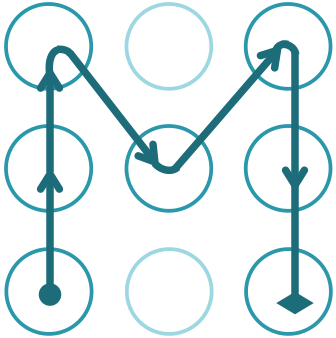
\includegraphics[width=0.27\textwidth]{pics/letters/bokstavenM.png}\hspace{0.6cm}
        }
        \subfigure[The letter N]{
          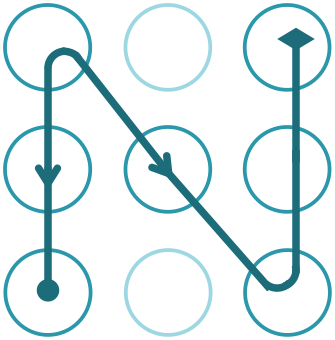
\includegraphics[width=0.27\textwidth]{pics/letters/bokstavenN.png}\hspace{0.6cm}
        }
        \subfigure[The letter O]{
          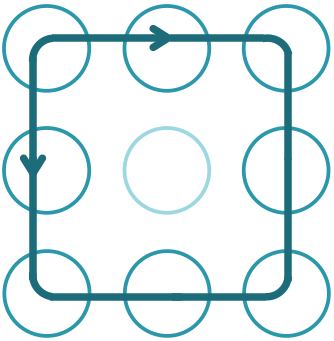
\includegraphics[width=0.27\textwidth]{pics/letters/bokstavenO.png}
        }

        \vspace{0.5cm}

        \subfigure[The letter S]{
          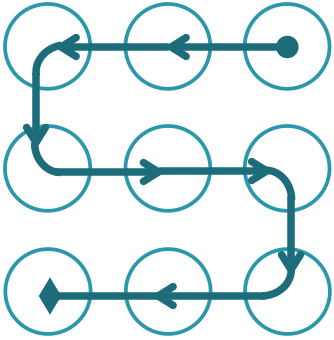
\includegraphics[width=0.27\textwidth]{pics/letters/bokstavenS.png}\hspace{0.6cm}
        }
        \subfigure[The letter U]{
          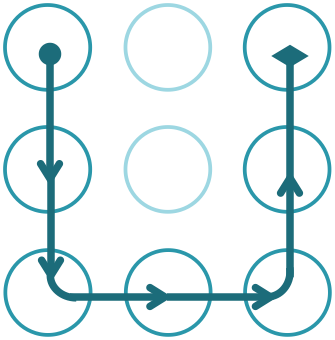
\includegraphics[width=0.27\textwidth]{pics/letters/bokstavenU.png}\hspace{0.6cm}
        }
        \subfigure[The letter Z]{
          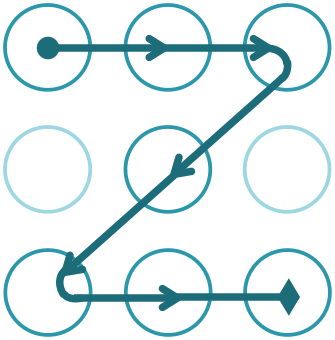
\includegraphics[width=0.27\textwidth]{pics/letters/bokstavenZ.png}
        }

        \vspace{0.5cm}
        \caption{Most frequent patterns forming letters from the alphabet}
        \label{fig:associationpatterns}
      \end{figure}

    \clearpage

  \subsection{Bias in the Selection of Start Node}
  
    The starting node of a pattern is a crucial information to have when analyzing patterns because of the properties of a legal pattern. A legal pattern can only visit the same node twice, making the starting point a help for excluding probable patterns.

    Table \ref{tab:startingNode1} is a summary of the likelihood of starting in a particular node for each of the four pattern types. The numbers notation used in the table, 1-3 and T, is a shortcut for the different pattern types shopping account (1), smartphone (2), banking account (3), and training (T). On average, 44\% of all patterns starts in node 1, e.g. the upper-left corner. Summarizing the most common starting points, node 1, 2 and 7, they all together constitutes 73\% of the patterns. 

    %Table: Starting node dist
    \begin{table}[H]
      \centering
      \begin{tabular}{ c || c | c || c | c | c | c }
        \hline
        {\bf Start node} & All & 1,2,3 & 1 & 2 & 3 & T \\ \hline
        1 & 44\% & 42\% & 43\% & 41\% & 42\% & 51\% \\
        3 & 15\% & 15\% & 16\% & 14\% & 13\% & 14\% \\
        7 & 14\% & 14\% & 13\% & 15\% & 14\% & 13\% \\
        2 & 9\%  & 9\%  & 10\% & 9\%  & 8\%  & 7\%  \\
        4 & 6\%  & 7\%  & 6\%  & 7\%  & 7\%  & 6\%  \\
        5 & 4\%  & 4\%  & 4\%  & 4\%  & 4\%  & 3\%  \\
        9 & 4\%  & 4\%  & 3\%  & 3\%  & 5\%  & 3\%  \\
        8 & 2\%  & 3\%  & 2\%  & 3\%  & 3\%  & 2\%  \\
        6 & 2\%  & 2\%  & 2\%  & 2\%  & 3\%  & 2\%  \\ \hline
      \end{tabular}
      \caption{Selection of starting node for all pattern types}
      \label{tab:startingNode1}
    \end{table}

    Figure \ref{fig:startingNode3} is an illustration of the likeliehood of starting in the different nodes. Each node has a number, starting from node 1 in the upper left corner ending up with node number 9 as shown in Figure \ref{fig:startingNode2}. All nodes in Figure \ref{fig:startingNode3} are colored based on the likeliehood of being chosen as a starting point from high to low (green - blue - orange), whereas the green nodes are the most common starting points and orange nodes is the least common starting points.

      %Figure: Staring node for all patterns
    \begin{figure}[H]
      \centering
      \subfigure[Node positions]{
        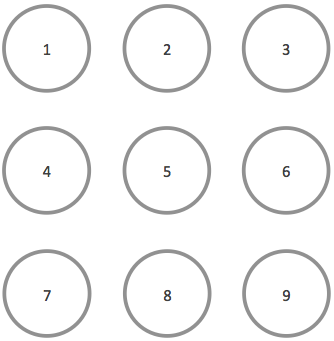
\includegraphics[scale=0.40]{pics/analysis/nodeposition.png}
        \label{fig:startingNode2}
      }
      \hspace{0.7cm}
      \subfigure[Staring node for all pattern types]{
        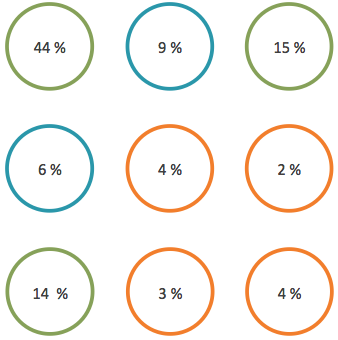
\includegraphics[scale=0.40]{pics/analysis/commonnode.png}
        \label{fig:startingNode3}
      }
      \caption{Node position and likely starting point for all pattern types}
      \label{fig:startingNode4}
    \end{figure}

  \subsection{3-gram Movement Patterns} \label{sec:3gram}
    
  %Figure: Most common 3-gram to less common 3-gram
  \begin{figure}[H]
    \subfigure{
      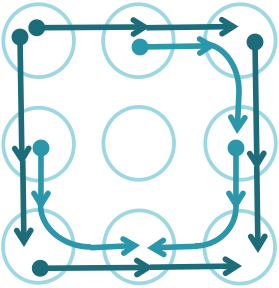
\includegraphics[width=0.31\textwidth]{pics/analysis/3gram1.png}
    }
    \subfigure{
      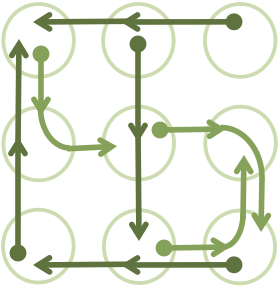
\includegraphics[width=0.31\textwidth]{pics/analysis/3gram2.png}
    }
    \subfigure{
      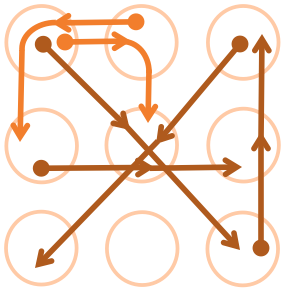
\includegraphics[width=0.31\textwidth]{pics/analysis/3gram3.png}
    }
    \caption{Most common 3-gram to less common 3-gram}
    \label{fig:3gram}
  \end{figure}
